\section{Benchmarks}
\label{sec:benchmark}

\subsection{Experiment system}
\label{sec:system}

Mira \cite{Chen:BGQ}, with 48 compute racks (48K nodes and 768K cores) at the ALCF, provides 10 PFlops theoretical peak performance. Each node has a 16-core processor and 16 GB of memory.

The interprocess communications of Blue Gene/Q travel on a 5D torus network both for point-to-point and for collective communications. This 5D torus interconnects a compute node with its 10 neighbors at 2 GB/s theoretical peak over each link in each direction, making a total of 40 GB/s bandwidth in both directions for a single compute node. Because of packet and protocol overheads, however, only up to 90\% of the raw data rate (1.8 GB/s) is available for user data. The machine can be partitioned into non-overlapping rectangular submachines; these submachines do not interfere with each other except for I/O nodes and the corresponding storage system.

For interconnect network traffic, BG/Q supports both deterministic and dynamic routing \cite{Chen:BGQ}. In the dynamic routing, messages in different message size ranges can be routed differently. However, within a given message size range, routing is always the same, and its path is known before it is routed. These are the default routing algorithms and cannot be changed during run time. The BG/Q supercomputer uses single-path data routing, for sending/receiving a message only one link of the ten available is used. The details of routing can be found in \cite{Chen:BGQ}.

PAMI is a low-level communication library for BG/Q \cite{PAMI:Kumar}. PAMI provides low-overhead communication by using various techniques such as accelerating communication using threads, scalable atomic primitives, and lockless algorithms to increase the messaging rate. Since MPI is implemented on top of PAMI, direct use of PAMI would provide higher messaging rates as well as lower latencies in comparison with MPI.




\subsection{Synthetic benchmarks}

%We carried our experiments on Mira, a Blue Gene/Q supercomputer. 
We evaluated our approaches on Mira, varying the partition size from 512 nodes to 4096 nodes. %The experiments involved a subset or the entire set of nodes for each partition. 
We varied the number of sources and destinations, and the average distance between them. 
We also experimented with different data sizes to be transferred. 
%We also varied the data sizes to be exchanged to find the effective data size.
We show results for various combinations of source-destination pairs. 
%Pairs of sources and destinations are randomized to show the efficacy of our work. 
The number of shortest paths used by our approaches was 50. % solvers to measure the effectiveness of number of paths to throughput. 
The maximum load $maxload$ for our heuristic approach was 16. 
%A similar benchmark with various max load is done for the heuristic approach. 
%For searching optimal paths we used AMPL (A Modeling Language for Mathematical Programming) and its solvers \cite{AMPL} for modeling our problem, and to find solutions for optimal data movement.


%\subsection{MPI Paths Reconstruction}

In our experiment we need to measure not only the performance of MPI routines, but also loads on physical links, and the number of hops per path that MPI takes to move data from a set of sources to a set of destination. The load and hops informatoon can reveal details on performance differences between MPI and our framework OPTIQ. Thus reconstructing MPI's paths is necessary to get load and hops information.

We reconstruct MPI's paths based on our understanding of default routing algorithms described in \cite{Chen:BGQ}. For each pair of source and destination we start at a source node and follow the rules of the routing algorithm to move data from the source node to its destination. We then record paths for all the pairs and use them to calculate load and number of hops.


\subsection{Communication Patterns}
In this paper we demostrate data movement performance of our OPTIQ framework and existing MPI's routines on the following communication patters:

\begin{figure}[ht]
\vspace{-0.1in}
\centering
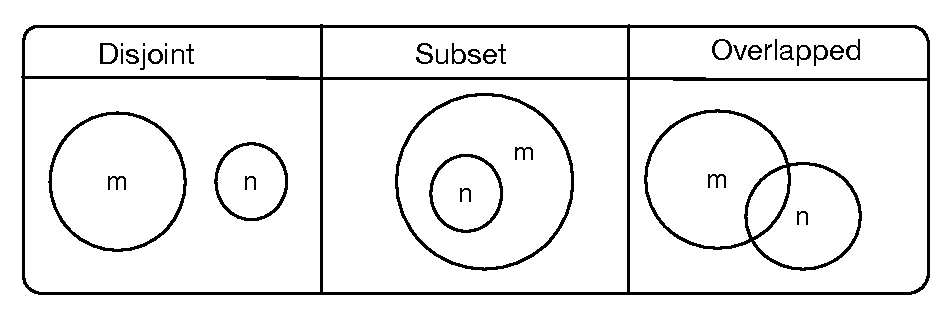
\includegraphics[scale=0.55]{figures/patterns.pdf}
\vspace{-0.1in}
\caption{Communication patterns}
\vspace{-0.1in}
\label{fig:patterns}
\end{figure}

\begin{itemize}
\item Disjoint sets: is many-to-many communication pattern where the sources and destinations are separated. It is a typical pattern in many applications.
\item Overlap: is a many-to-many pattern that sources and destinations are overlapped sets. CESM uses this communication patterns for its coupling communications.
\item Subset: is a many-to-many pattern that sources or destinations are subset of the other. The patterns can be found CESM or in I/O aggregation.
\end{itemize}

We carried a set of experiments to study the system's behavior in various patterns and demontrate throughput improvement.


\subsection{Experiments and Results}

We carried out a set of experiments and measured the follows: throughput of data transfer, total number of paths found, number of paths per pair of source-destination (a job), hopbytes (multiplication of an amount of data and a number of hops it travels on a path) values on a path, number of paths that shares a physical link, and amount data that passes through a physical link. We used our framework OPTIQ and MPI\_Alltoallv to transfer data and compare 2 ways to show the efficacy of our framework. MPI\_Alltoallv is typical way to transfer data between a set of sources and a set of destinations. It uses default routing algorithms i.e. both dynamic and static routing can be employed.

\subsubsection{Varying partition, source and destination sizes, keeping the same sources/destination ratio}

\begin{figure*}[!htbp]
        \centering
        \begin{subfigure}[b]{0.32\textwidth}
                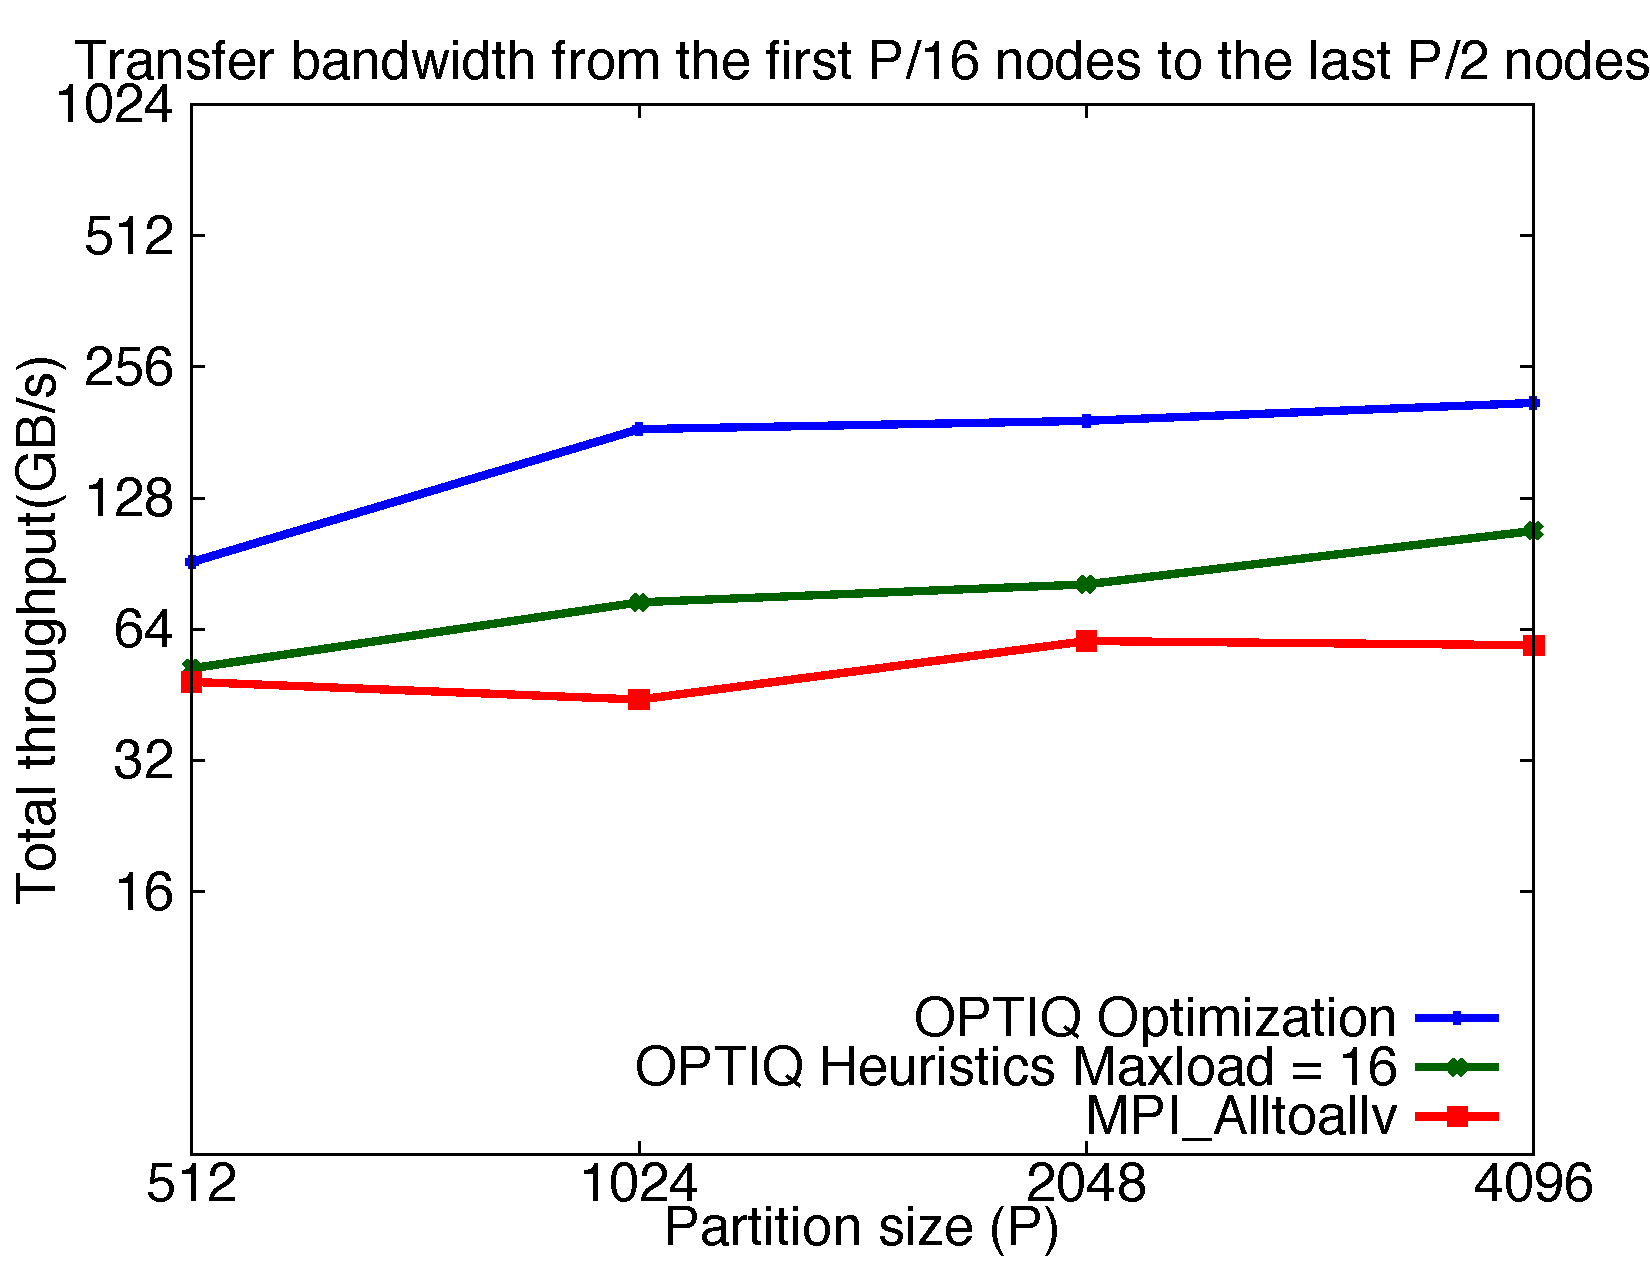
\includegraphics[width=\textwidth]{figures/constantr_3.pdf}
                \caption{Disjoint}
                \label{fig:constantr_3}
        \end{subfigure}%
        ~ %add desired spacing between images, e. g. ~, \quad, \qquad, \hfill etc.
          %(or a blank line to force the subfigure onto a new line)
        \begin{subfigure}[b]{0.32\textwidth}
                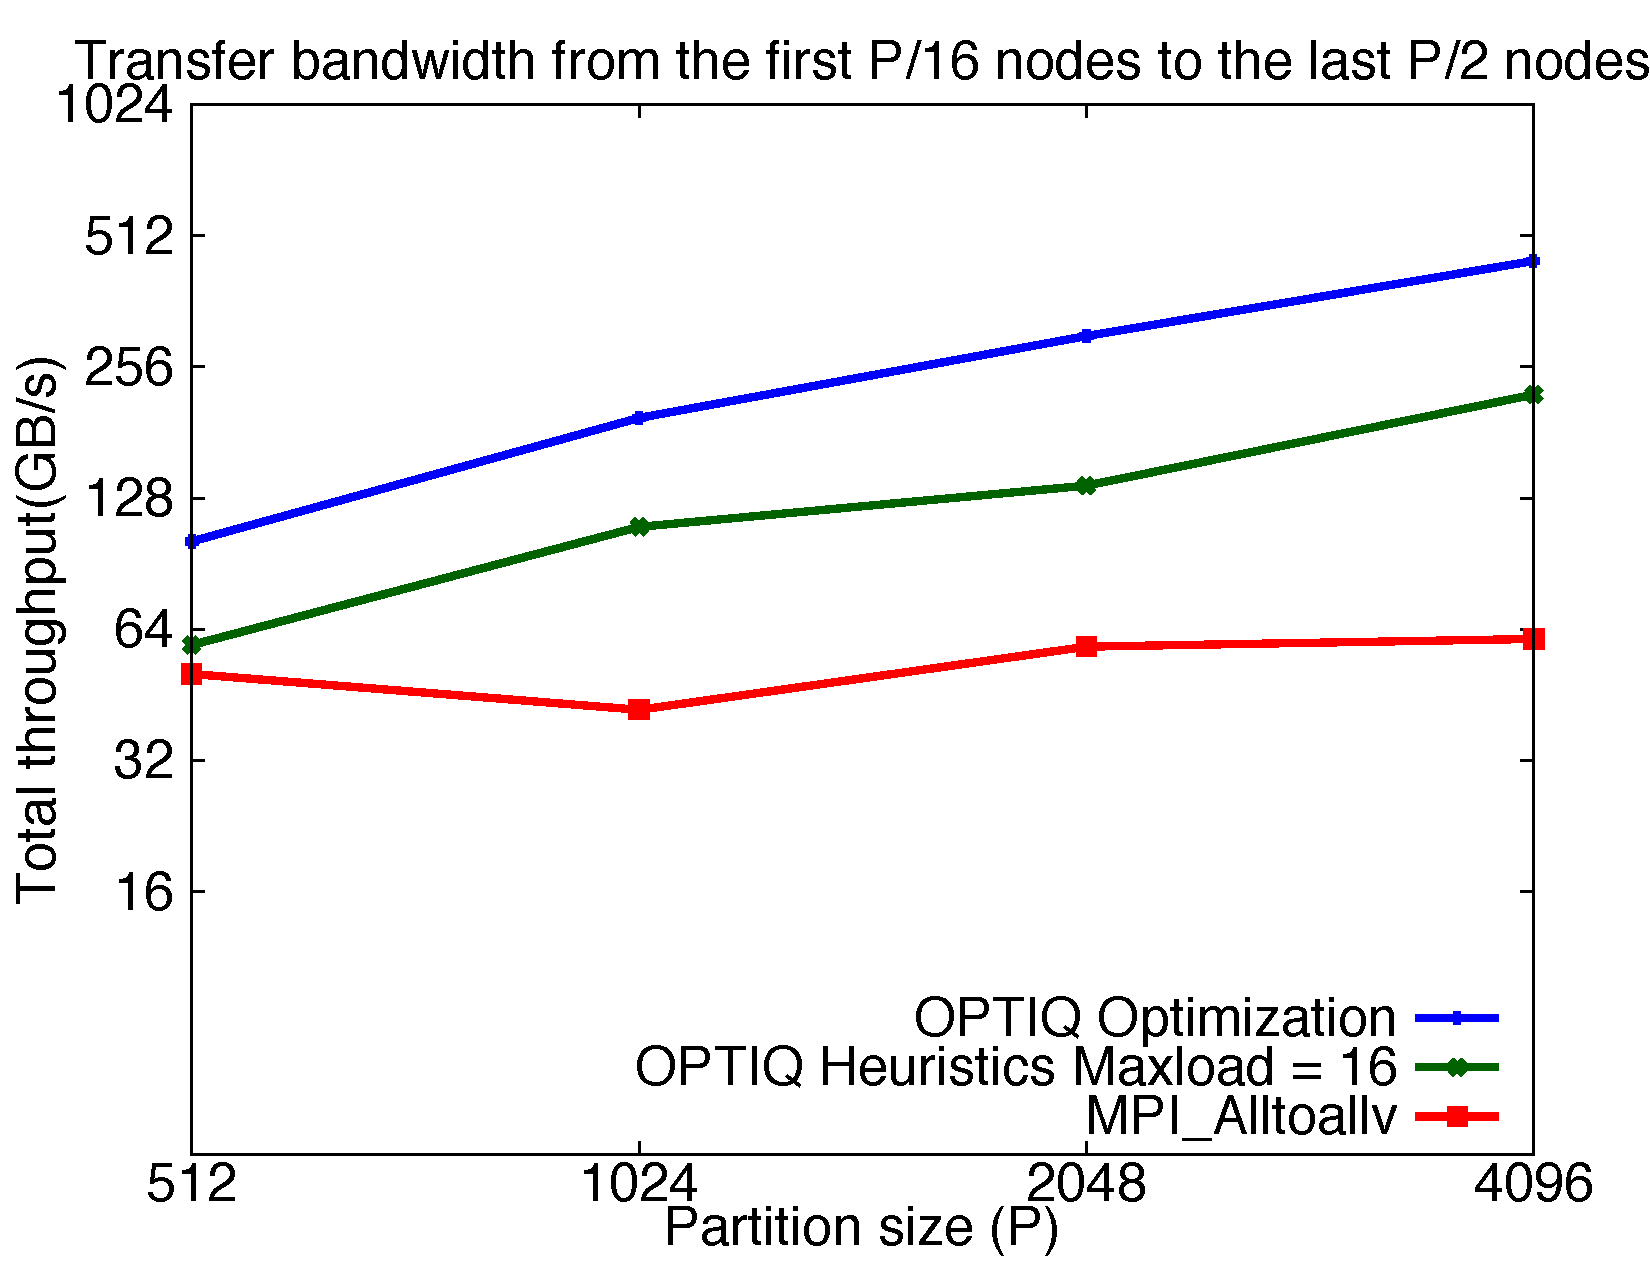
\includegraphics[width=\textwidth]{figures/constantr_27}
                \caption{Overlap}
                \label{fig:constantr_27}
        \end{subfigure}
        ~ %add desired spacing between images, e. g. ~, \quad, \qquad, \hfill etc.
          %(or a blank line to force the subfigure onto a new line)
        \begin{subfigure}[b]{0.32\textwidth}
                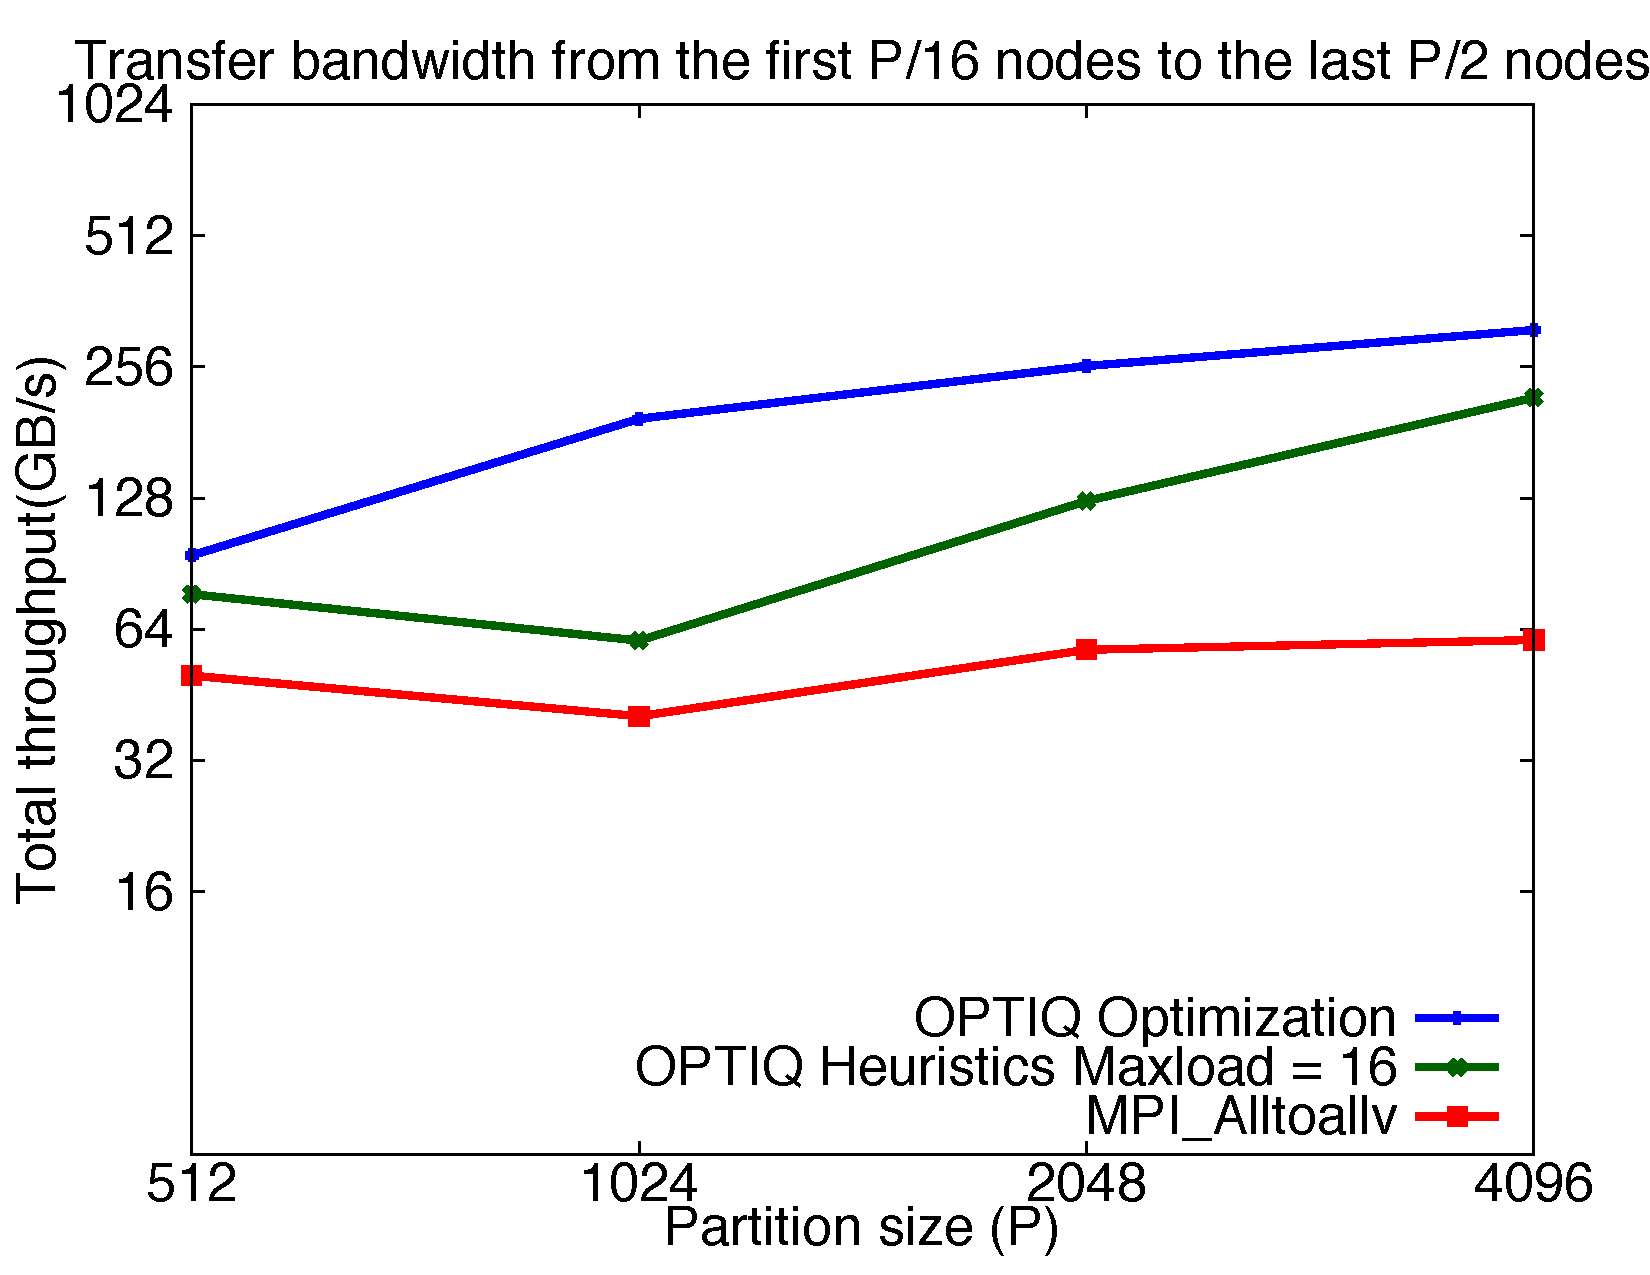
\includegraphics[width=\textwidth]{figures/constantr_87}
                \caption{Subset}
                \label{fig:constantr_87}
        \end{subfigure}
        \caption{Varying the number of sources and destinations and total number of nodes while keeping the ratio constant (1:8).}
        \label{fig:constantr}
\end{figure*}

\begin{table*}[!htbp]
   \centering
    \begin{tabular}{| l | l | r | r | p{0.5cm} | p{0.5cm} | p{0.5cm} | p{0.5cm} |p{0.5cm} | p{0.5cm} |p{0.5cm} | p{0.5cm} |p{0.5cm} | p{0.5cm} |}
    \hline
    \multirow{3}{*}{Pattern} & \multirow{3}{*}{Type} & \multirow{3}{1cm}{BW (GB/s)} & \multicolumn{3}{ c| }{Num. of Paths} & \multicolumn{2}{ c| }{Hopbytes} & \multicolumn{2}{ c| }{Num of copies}& \multicolumn{2}{ c| }{Num of paths} & \multicolumn{2}{ c| }{Total data} \\ \cline{4-6}
    & & & \multirow{2}{0.5cm}{Total Paths} & \multicolumn{2}{ c| }{Per Job} & \multicolumn{2}{ c| }{Per Path (MB)} & \multicolumn{2}{ c| }{Per Path}& \multicolumn{2}{ c| }{Per Link}& \multicolumn{2}{ c| }{Per Link (MB)} \\ \cline{5-14}
    & & & & {Max} & Avg & Max & Avg & Max & Avg & Max & Avg & Max & Avg\\ \hline
    \multirow{3}{*}{Disjont} & OPT    & 188.62 & 1,169 & 6 & 2.28 & 83.88 & 23.02 & 1152 & 295.22 & 11 & 2.53 & 18.28 & 9.26 \\ \cline{2-14}
    & HEU & 74.88  & 3,146 & 23 & 6.14 & 83.88 & 8.45 & 1152 & 108.24 & 16 & 4.94 & 63.04 & 6.92 \\ \cline{2-14}
    & MPI    & 45.18  & 512  & 1 & 1.00 & 92.27 & 50.33 & & & 16 & 3.07 & 134.21 & 25.76\\ \hline
    \multirow{3}{*}{Overlap} & OPT    & 200.03 & 1303 & 6 & 2.54 & 83.88 & 19.28  & 1152 & 243.96 & 13 & 2.74 & 16.97 & 9.04\\ \cline{2-14}
    & HEU & 113.17  & 3273 & 26 & 6.39 & 75.49 & 7.41 & 1024 & 93.07 & 16 & 5.17 & 38.66 & 7.04 \\ \cline{2-14}
    & MPI    & 42.84 & 512 & 1 & 1.00 & 83.88 & 42.99 &  & & 16 & 3.38 & 134.21 & 28.36 \\ \hline
    \multirow{3}{*}{Subset} & OPT    & 199.20 & 1269 & 6 & 2.48 & 75.49 & 19.48 & 1024 & 245.66 & 11 & 2.79 & 17.10 & 9.32 \\ \cline{2-14}
    & HEU &  61.71 & 3238 & 26 & 6.32 & 75.49 & 7.43 & 1024 & 93.22 & 16 & 5.28 & 45.08  & 7.35 \\ \cline{2-14}
    & MPI    &  41.37 & 512  & 1 & 1.00 & 83.88 &  41.94 & & & 16 & 3.52 & 134.21 & 29.49 \\ \hline
    \end{tabular}
    \caption{Throughput, total num of paths, number of paths per job, maximum and average values of hopbytes, number of copies, number of paths per link and amount of data per link for 3 patterns in 1024 nodes experiments.}
    \label{table:constantr}
\end{table*}

\begin{figure}[!htb]
\vspace{-0.1in}
\centering
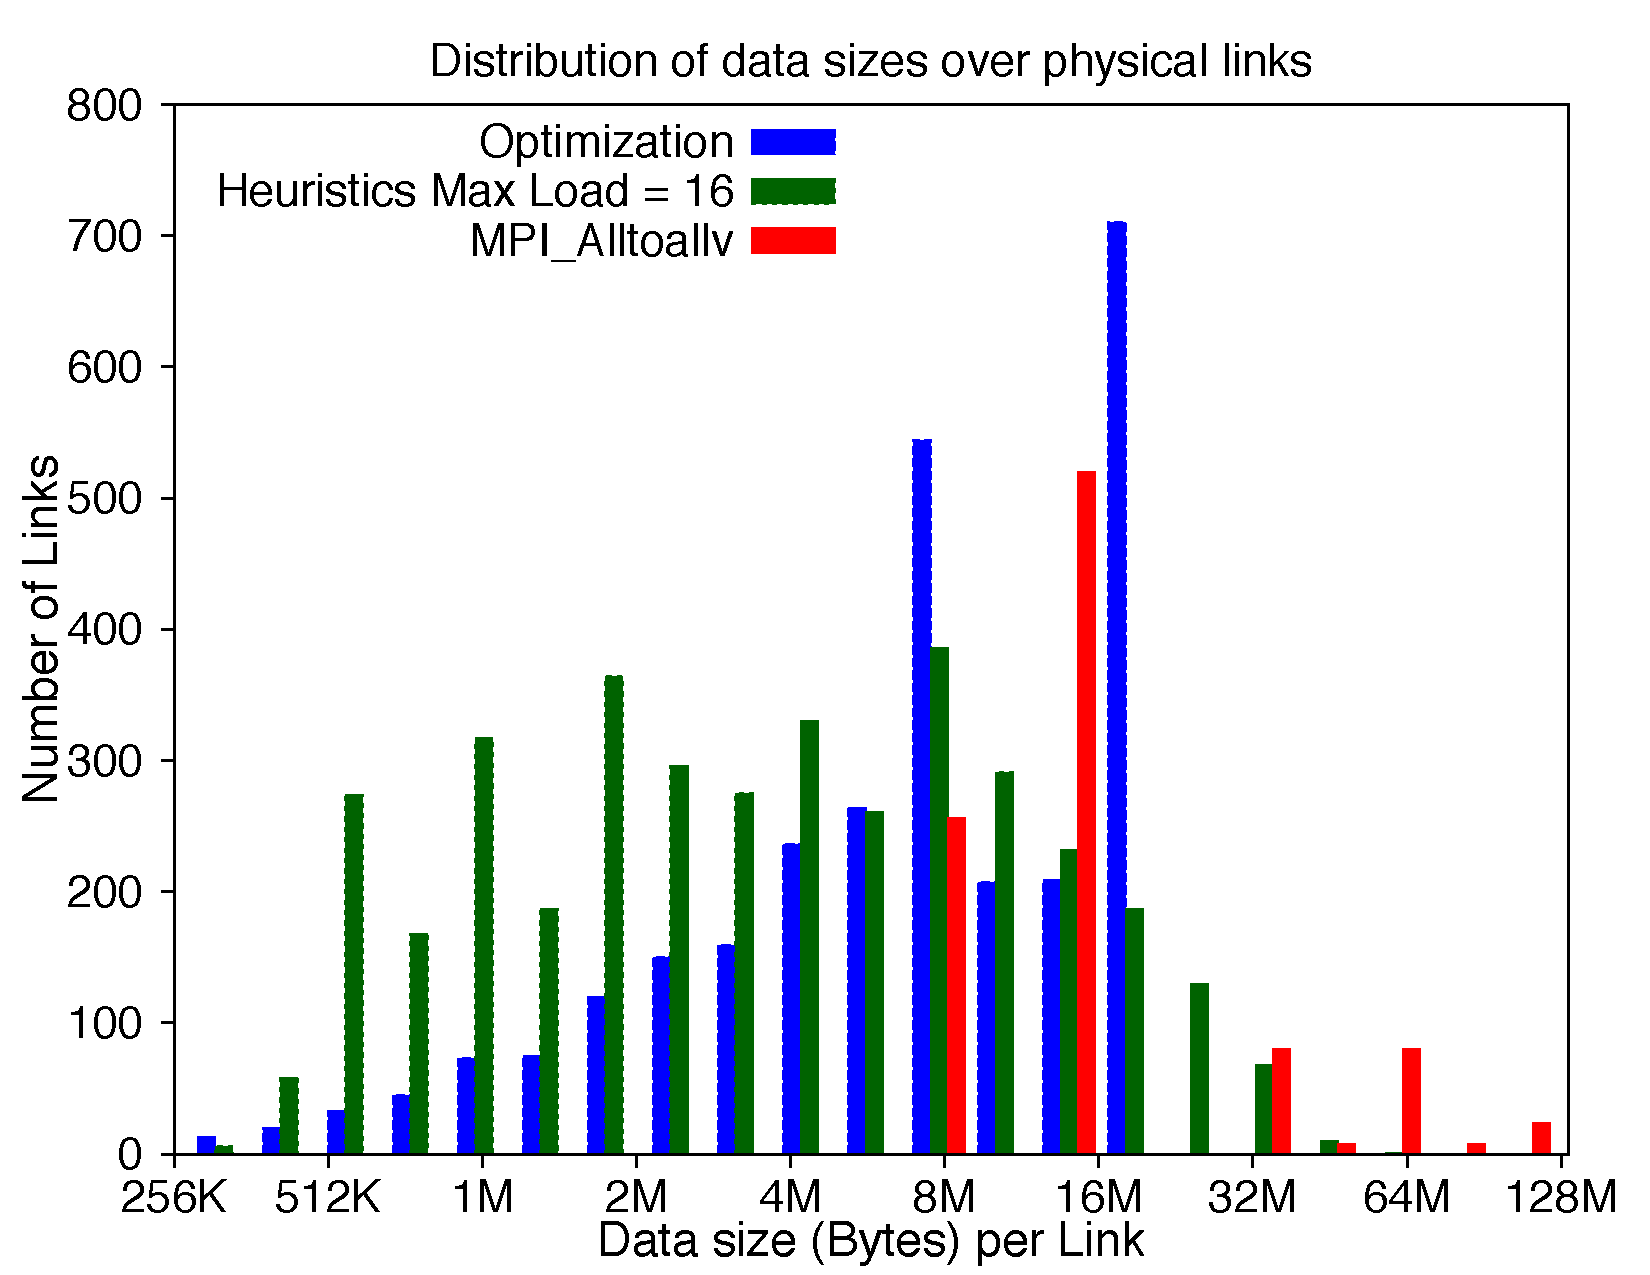
\includegraphics[scale=0.30]{figures/loaddata_histo.pdf}
\vspace{-0.1in}
\caption{Distribution of total amount of data per link for Disjoint pattern in 1024-node partition.}
\vspace{-0.1in}
\label{fig:loaddata_histo}
\end{figure}

\begin{figure}[!htb]
\vspace{-0.1in}
\centering
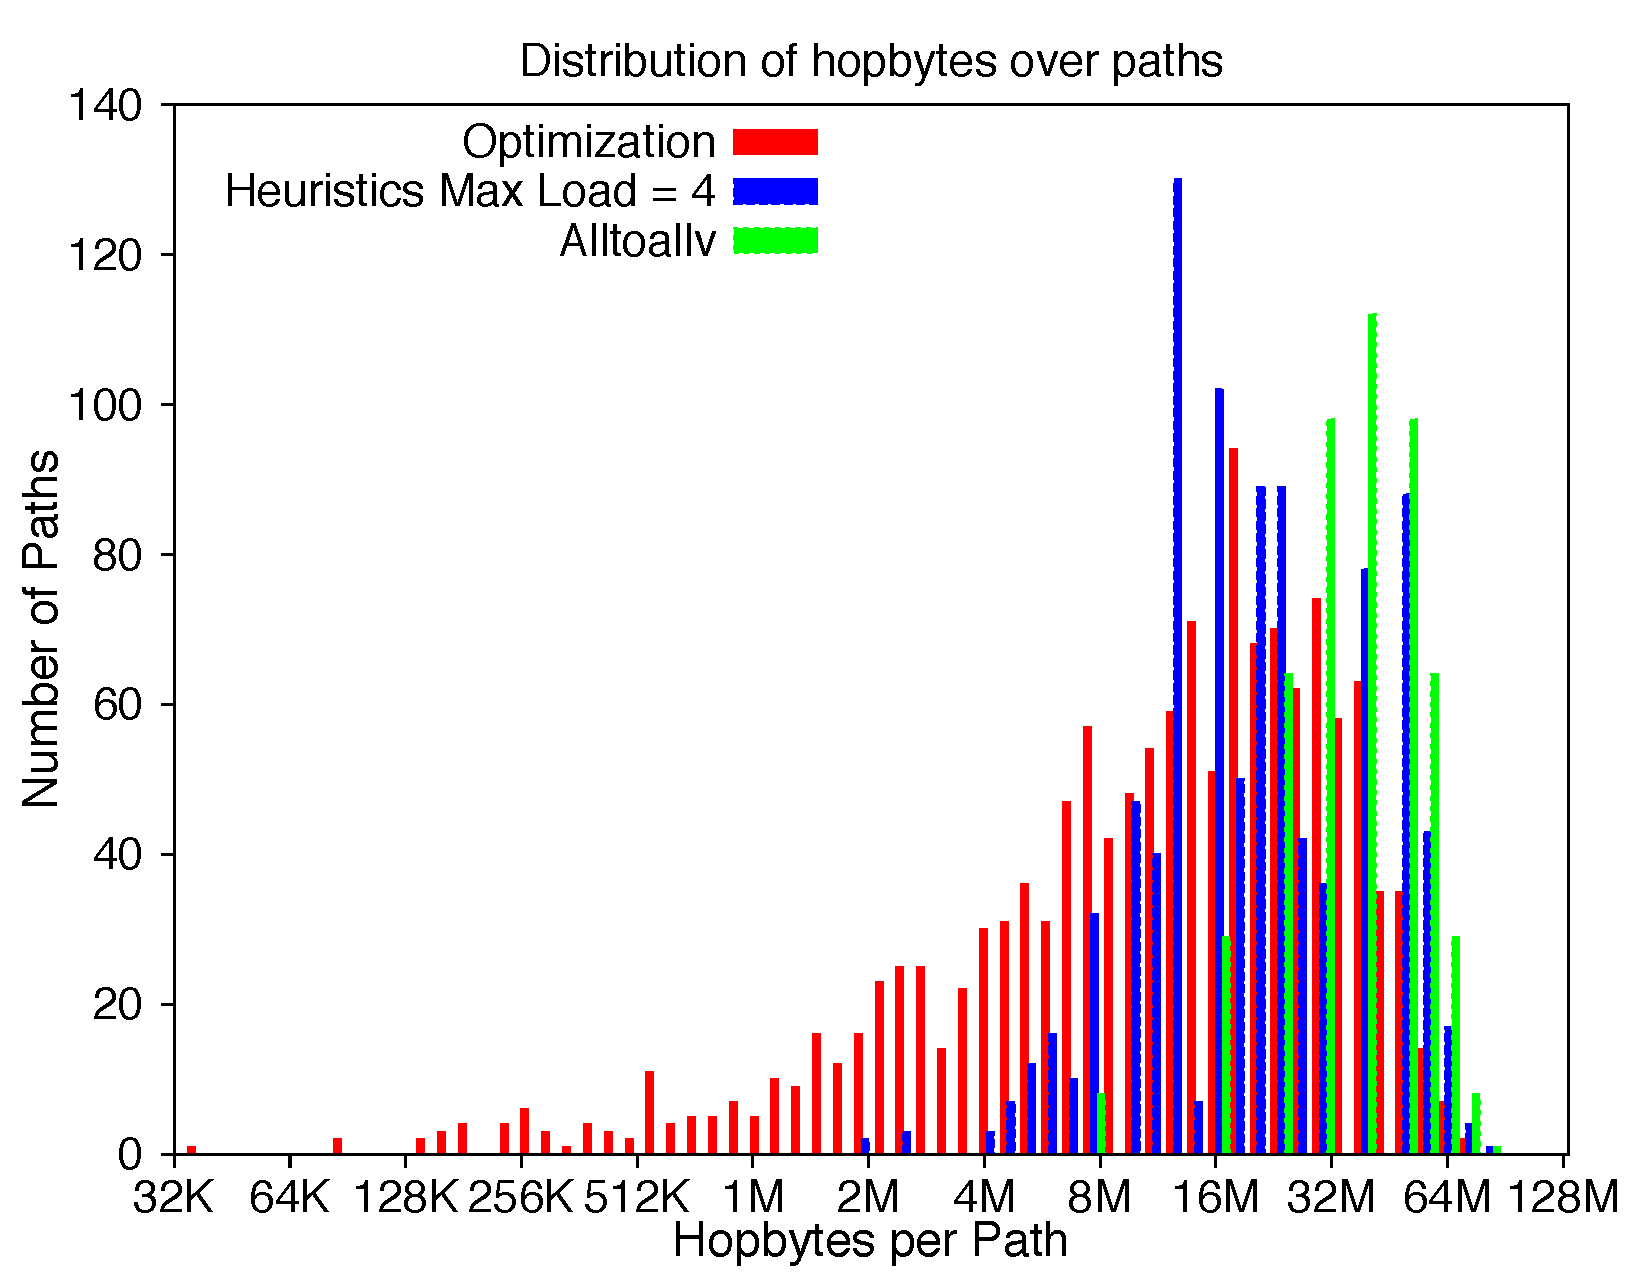
\includegraphics[scale=0.30]{figures/hopbyte_histo.pdf}
\vspace{-0.1in}
\caption{Distribution of hopbytes per path for Disjoint pattern in 1024-node partition.}
\vspace{-0.1in}
\label{fig:hopbyte_histo}
\end{figure}

In this experiment we vary the number of sources and destinations together with total number of nodes while keeping the ratio between the number of sources and destination at 1/8. While the total number of nodes P  increases from 512 to 4096 the first P/16 nodes send data to the last P/2 nodes. Each source has 8 destinations e.g node 0 sends data to nodes P/2, P/2+1, ...P/2+7. We tested the framework for 3 patterns: subset, disjoint and overlap, with 3 approaches of transferring data OPTIQ Optimization, OPTIQ Heuristics and MPI\_Alltoallv. We use 1 MPI/PAMI rank/node. The data size is 8 MB per pair. We set the $maxload$ to 16 for the Heuristic approach.

As shown in Figure \ref{fig:constantr} the Optimization approach has the highest throughput, the Heuristics approach is next and MPI\_Alltoall achieved the lowest throughput. The Table \ref{table:constantr} shows that in all three patterns the Heuristic with $maxload$ set to 16 was able to find highest number of paths. The Heurisc approach also has the highest maximum and average number paths for a job. As data is divided equally among paths, this led to lowest maximum and average values for hopbytes, number of copies per path. However this led to higher number of paths per physical link, and higher amount of data per physical link in the Heuristic approach in comparison to the Optimization approach. In Optimization the data is split among the paths to balance the amount of data between physical links, thus it has the lowest maximum amount of data per physical link. The distribution of the total amount of data in Figure \ref{fig:loaddata_histo} also shows this effect. This led to its highest throughput. MPI\_Alltoall approach has the lowest number of paths. With 1 path per pair of communication, data is not split. Thus it has the the highest hopbytes per path and amount of data per physical link. The distribution of its total data size per link in Figure \ref{fig:loaddata_histo} and its hopbytes per paths in Figure \ref{fig:hopbyte_histo} also show the effects. Both factors led to its lowest throughput.


\subsubsection {Three communication patterns with random message sizes}
In this experiment, we varied the number of source nodes, number of destination nodes and total number of nodes (partition sizes) but kept the ratio between the source nodes and the destination nodes constant. With P is size of the partition, we choose the first P/16 nodes as the source nodes, and N/2 last nodes as the destination nodes. Each node in the set of source nodes communicates with 8 nodes in the set of destination nodes. The pairing is aligned i.e. node 0 communicates with nodes (P/2, ..., P/2/7). We randomly choosing the data size for each pair of communication from 64 KB up to 8 MB of data. We experimented with 3 communication patterns: Disjoint, Overlap, Subset and 3 approaches: Optimization, Heuristic and MPI\_Alltoallv. We used only 1 MPI/PAMI rank per node. The total number of nodes P varied from 512 up to 4096 nodes. The communication throughputs are shown in Figure \ref{fig:constantr_msg}.

\begin{figure*}[!htbp]
        \centering
        \begin{subfigure}[b]{0.32\textwidth}
                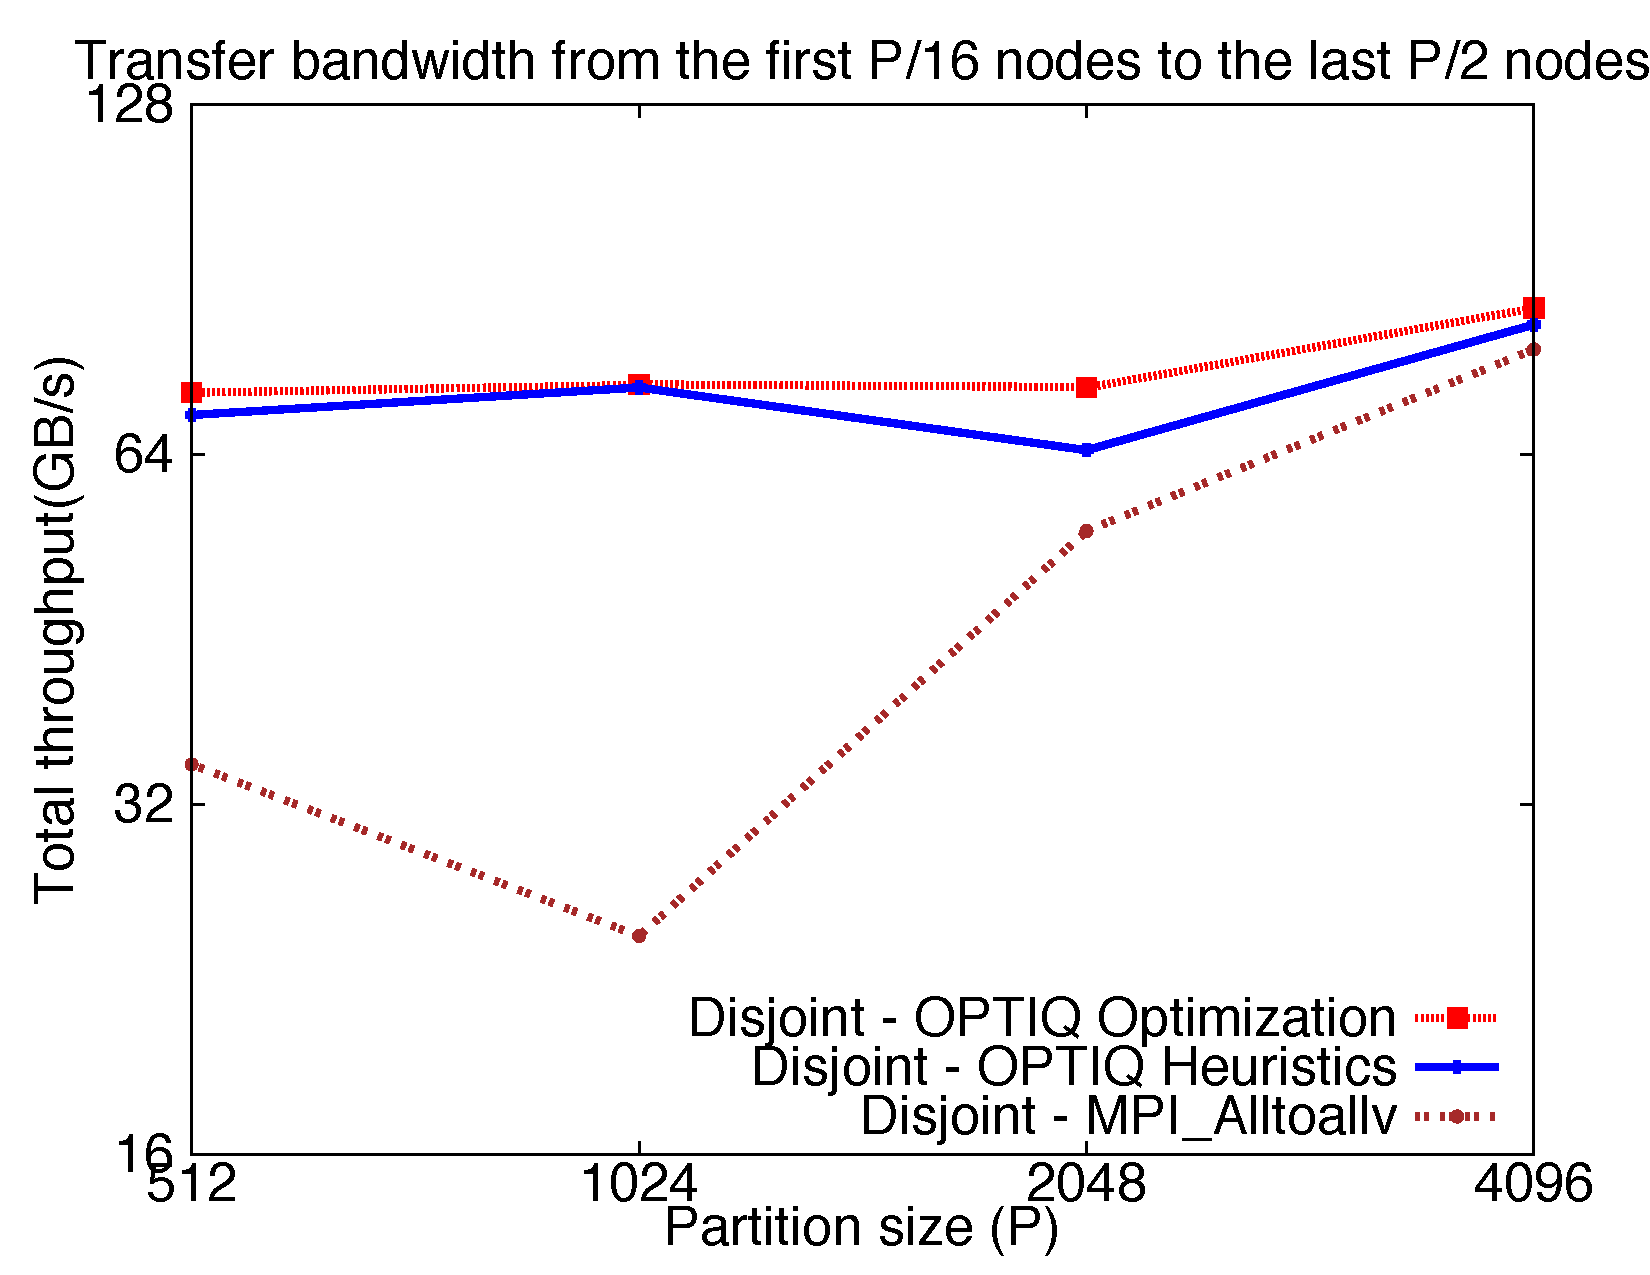
\includegraphics[width=\textwidth]{figures/constantr_disjoint_msg.pdf}
                \caption{Disjoint}
                \label{fig:constantr_disjoint_msg}
        \end{subfigure}%
        ~ %add desired spacing between images, e. g. ~, \quad, \qquad, \hfill etc.
          %(or a blank line to force the subfigure onto a new line)
        \begin{subfigure}[b]{0.32\textwidth}
                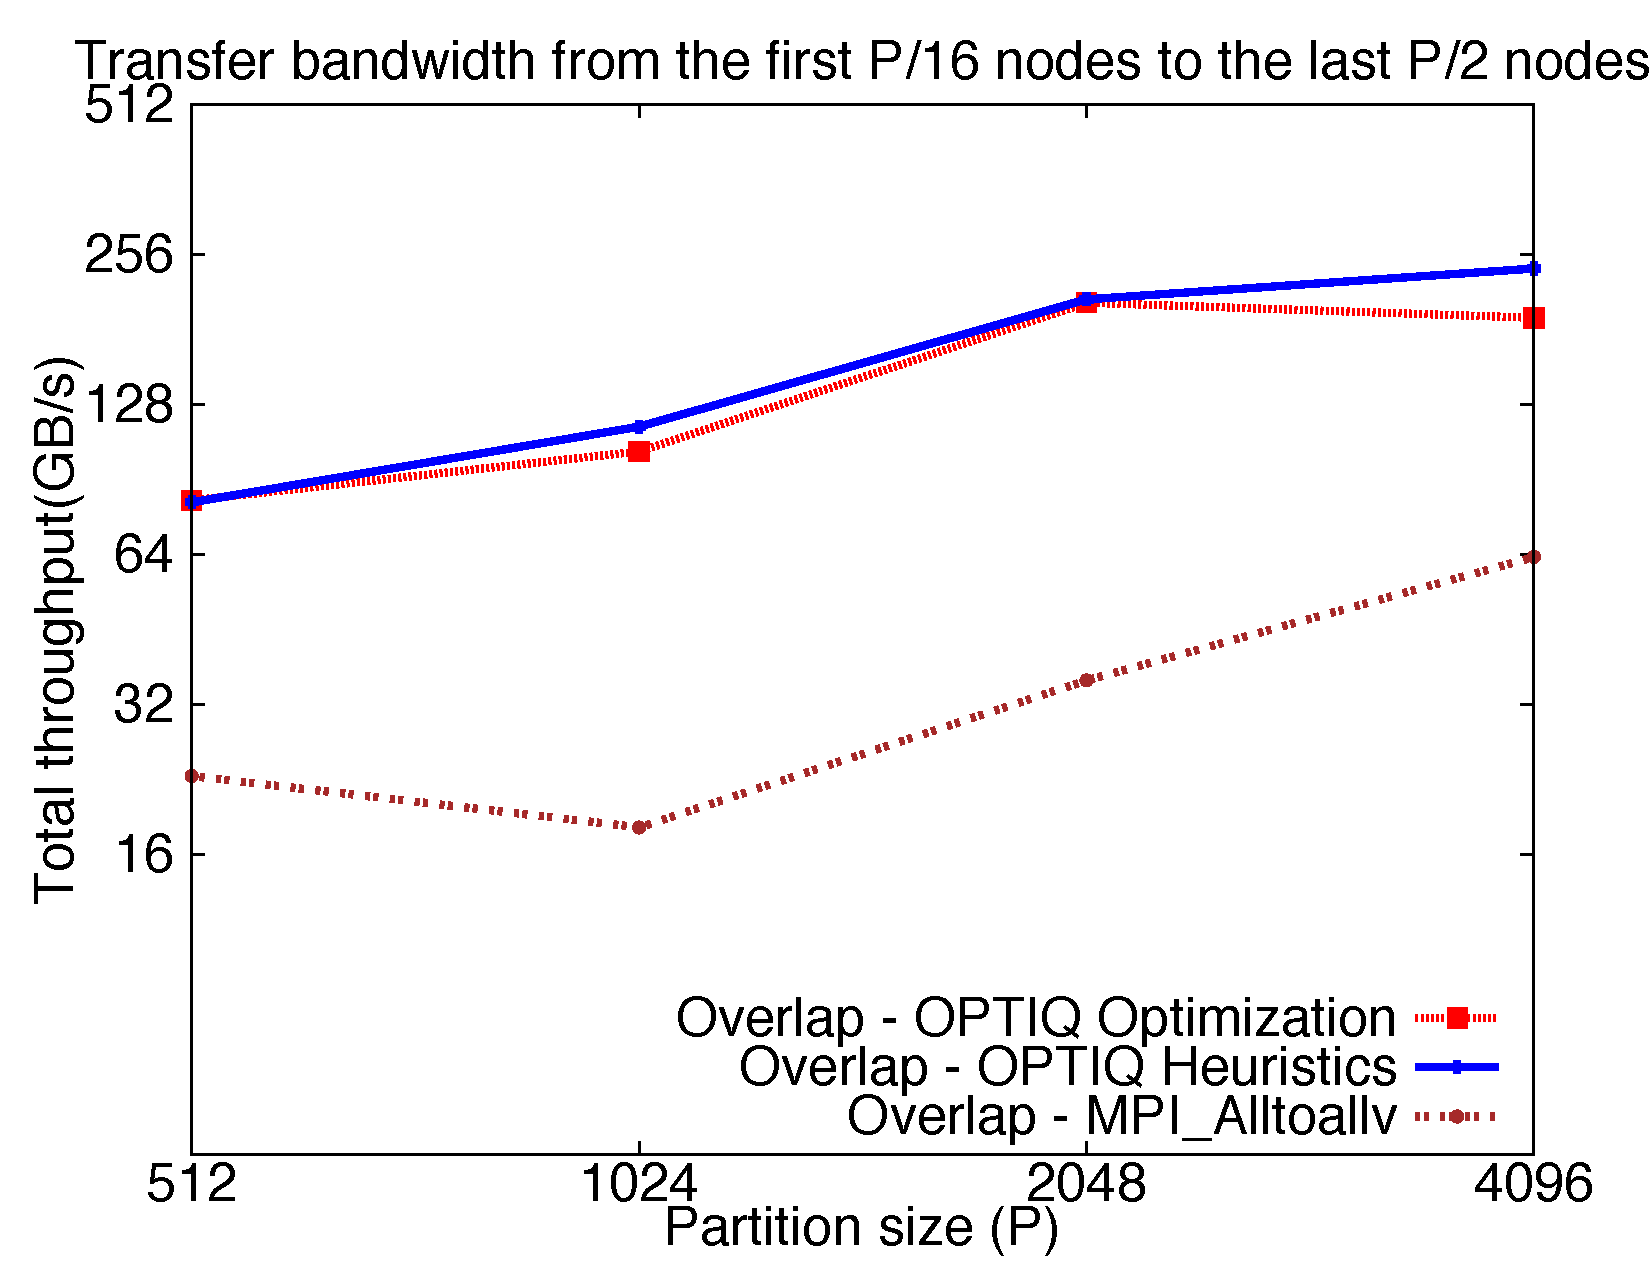
\includegraphics[width=\textwidth]{figures/constantr_overlap_msg.pdf}
                \caption{Overlap}
                \label{fig:constantr_overlap_msg}
        \end{subfigure}
        ~ %add desired spacing between images, e. g. ~, \quad, \qquad, \hfill etc.
          %(or a blank line to force the subfigure onto a new line)
        \begin{subfigure}[b]{0.32\textwidth}
                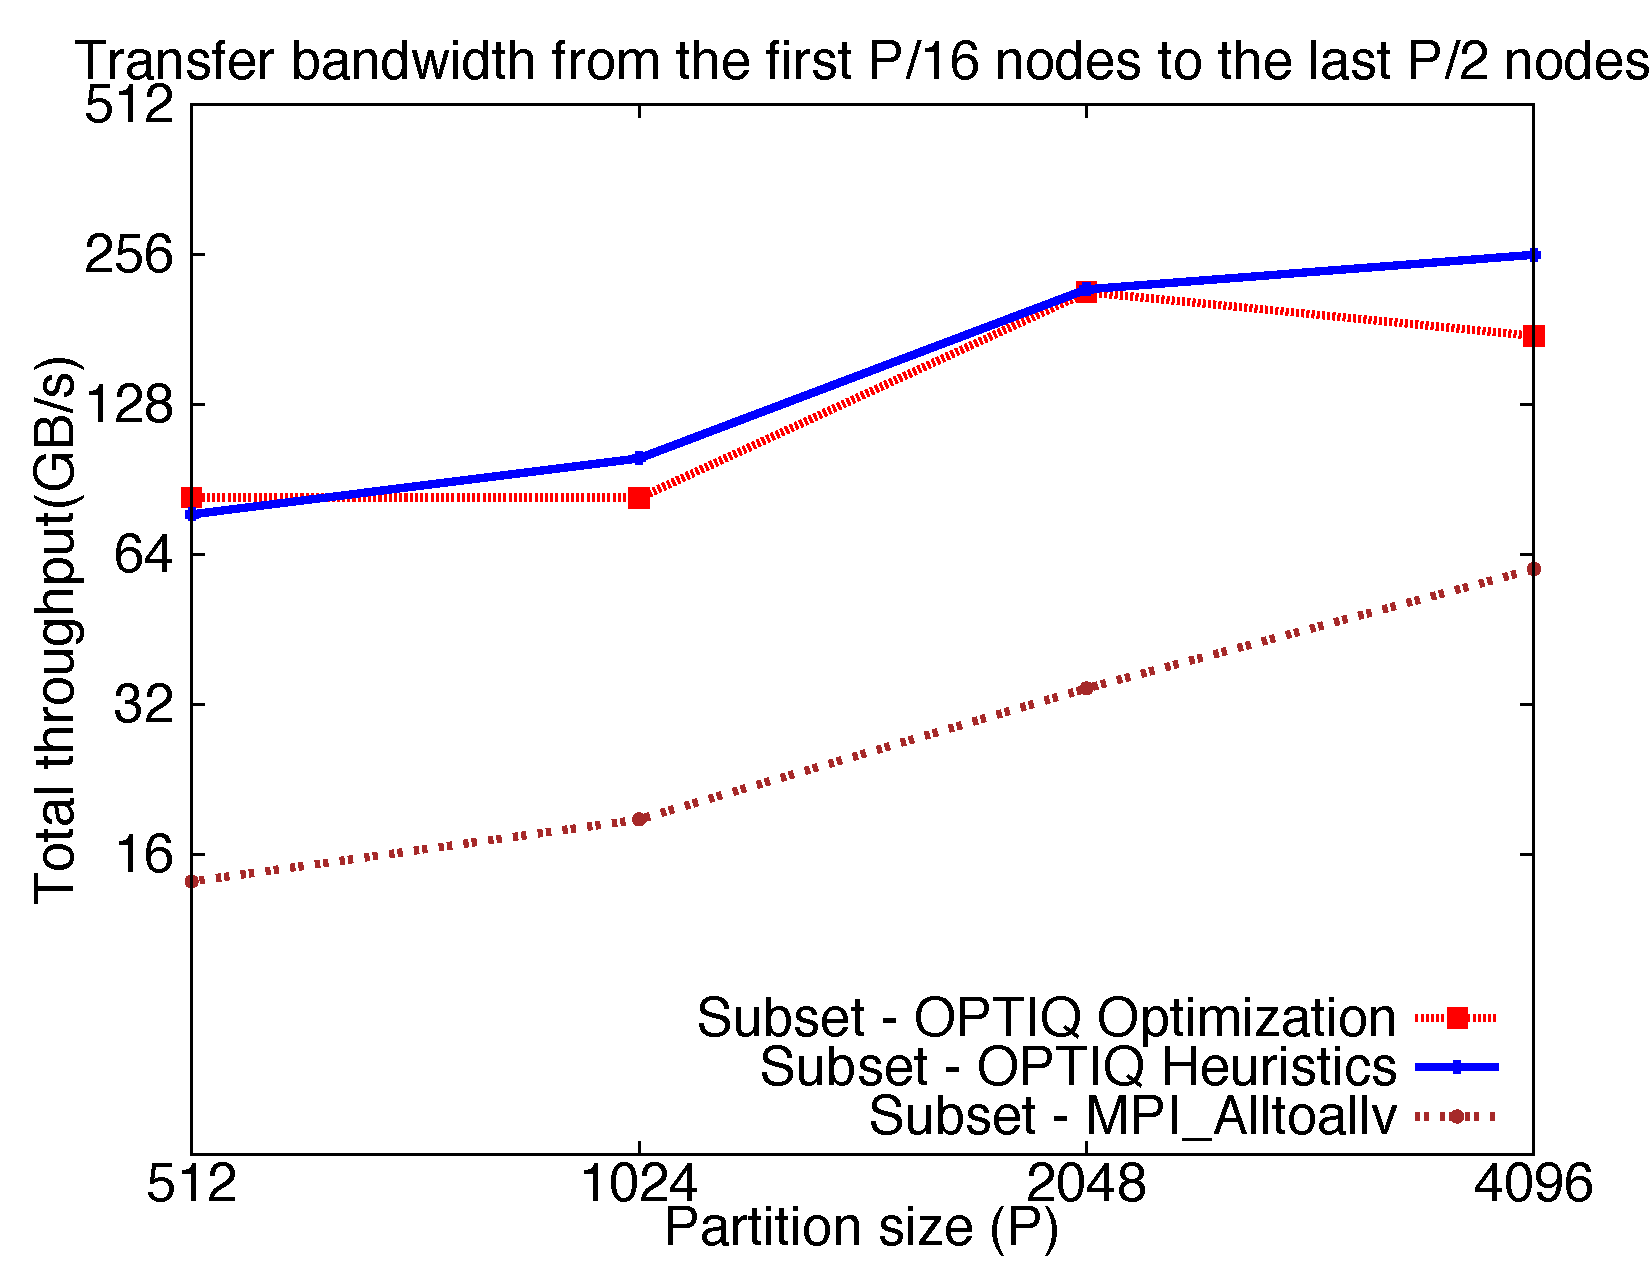
\includegraphics[width=\textwidth]{figures/constantr_subset_msg.pdf}
                \caption{Subset}
                \label{fig:constantr_subset_msg}
        \end{subfigure}
        \caption{Varying the number of sources and destinations and total number of nodes with constant ratio}
        \label{fig:constantr_msg}
\end{figure*}

As shown in the Figure \ref{fig:constantr_msg}, in all the three communication patterns, Optimization approach and Heuristic approach have similar performance and is both significant higher than MPI\_Alltoallv in most of the experiments. In Disjoint pattern, the performance gap is close at 4096 nodes with at the other 2 patterns, the gap is quite constant showing the scalability of our approaches.

In the next section, we demonstrate the efficacy of our approaches through an experiment with communication patterns and data from a real application Community Earth System Model (CESM).


%\subsubsection {Multiple ranks}
%In this experiment, we demonstrate the scalability of our framework when increasing the number of MPI/PAMI ranks per node.

